\documentclass{beamer}
\usepackage{pgf,tikz}
\usepackage[french]{babel}
\usetikzlibrary{arrows}
\usepackage[utf8]{inputenc}
\usepackage[T1]{fontenc}
\usepackage{lmodern}
\usepackage{enumerate}
\usepackage{amsmath, amssymb, amsthm}
% for use in integrals and derivatives
\newcommand{\dd}{\mathrm d}
\usepackage{hyperref}
\usetheme{Warsaw}
\usefonttheme{professionalfonts}
\setbeamertemplate{navigation symbols}{}
\setbeamertemplate{headline}{}
\setbeamertemplate{footline}{}

\title{Observation de débris spatiaux}

\author{Nicolas Bonnotte, Maxime Chupin, Tony Février, Antoine Levitt,
  Benjamin Marteau, Vladimir Salnikov\\\vspace{1cm}Sujet proposé par Max Cerf, EADS}

\date{19 octobre 2012}
\institute{SEME 4, Institut Henri Poincaré}

\renewcommand{\leq}{\leqslant}
\renewcommand{\le}{\leqslant}
\renewcommand{\geq}{\geqslant}
\renewcommand{\ge}{\geqslant}

\begin{document}

\AtBeginSection[]
{
  \begin{frame}
    \tableofcontents[currentsection]
  \end{frame}
}

% \newcommand{\OutlineColumnNumbers}{2}

\frame{\titlepage}
\section{Introduction}
% Historique débris


\section{Introduction}

Micrométéorites,
%écailles de peinture détachée d'un engin spatial, 
petites pièces relâchées lors de la séparation de deux étages d'une fusée, 
débris produits par la collision d'un vieux satellite avec d'autres débris... 
l'espace en orbite basse est plein de petits objets, qui représentent un danger permanent pour le matériel et pour les hommes qui s'y trouvent.
Leur danger vient de leur vitesse, 7 ou 8~km/s, et de leur nombre : la \textsc{nasa} estime à plus de 21~000 le nombre de débris de plus de 10~cm, et à plus de de 500~000 les débris ayant entre 1 et 10~cm de diamètre\footnote{Source : \url{http://orbitaldebris.jsc.nasa.gov/faqs.html}. Notons qu'un tiers de tous les débris ont été créés par la destruction volontaire d'un vieux satellite par un missile chinois, en 2007, et par la collision accidentelle d'un satellite américain et d'un satellite russe en 2009.}. Il est donc éminemment nécessaire de pouvoir les détecter.

Ces débris peuvent être repérés depuis le sol. Mais comment faire pour en détecter le plus possible, tout en minimisant naturellement le coût pour le faire ? Tel est le problème que Max Cerf (\textsc{eads}--Astrium) nous a posé, lors de la 4\ieme{} 
Semaine d'étude mathématiques et entreprises (\textsc{seme}), qui s'est tenue à
dans les locaux de l'Institut Henri Poincaré (\textsc{ihp}) à Paris du lundi 15
au vendredi 19 octobre 2012.  Plusieurs aspects contribuent à rendre ce problème difficile :
\begin{enumerate}
\item Les débris évoluant sur des orbites différentes, la latitude du télescope influe fortement sur le nombre d'orbites traversées par le champ de vision ;
\item Le nombre de débris que l'on peut observer sur une orbite donnée dépend aussi du temps pendant lequel cette orbite reste visible lorsqu'elle passe dans le champ de vision ;
\item Pour pouvoir observer un débris, encore faut-il qu'il soit éclairé par la lumière du soleil, et que le détecteur ne soit pas lui-même ébloui, c'est-à-dire qu'il faut qu'il fasse nuit pour lui ;
\item Enfin, la période de révolution d'un débris modifie la probabilité qu'il puisse être observé, suivant qu'il est plus ou moins synchronisé avec le détecteur.
\end{enumerate}

Les deux premiers aspects ont été étudiés dans la section~2, le troisième dans la section~3, le dernier dans la section~4. Dans la section~5, des simulations numériques donnent des résultats directs, indépendamment de la modélisation des aspects précités.
\paragraph*{Remerciements}

Le groupe souhaite remercier les organisateurs de la \textsc{seme}, ainsi que Astrium et plus précisément Max
Cerf pour avoir proposé ce sujet, que nous avons trouvé riche et intéressant.
\frame{\tableofcontents}
% \section{Probabilité d'observation}
% \frame{
%   \frametitle{Observation du débris}
%   \begin{itemize}
%   \item On ignore l'éclairage pour l'instant
%   \end{itemize}
%   \begin{center}
%   \resizebox{0.6\textwidth}{!}{ \newlength{\unit}
\newlength{\width}
\setlength{\width}{\figurewidth}
\setlength{\unit}{0.0926\width}
%\setlength{\unit}{1cm}
%\setlength{\unit}{\texwidth}

\definecolor{xdxdff}{rgb}{0.49,0.49,1}
\definecolor{qqwuqq}{rgb}{0,0.39,0}
\definecolor{qqqqcc}{rgb}{0,0,0.8}
\definecolor{qqqqff}{rgb}{0,0,1}
\begin{tikzpicture}[line cap=round,line join=round,>=triangle 45,x=\unit,y=\unit]
\clip(4.11,-0.63) rectangle (10.8,5.62);
\draw [shift={(5,3)},color=qqwuqq,fill=qqwuqq,fill opacity=0.1] (0,0) -- (49.79:0.75) arc (49.79:90:0.75) -- cycle;
\draw [shift={(5,0)},color=qqwuqq,fill=qqwuqq,fill opacity=0.1] (0,0) -- (72.58:0.75) arc (72.58:90:0.75) -- cycle;
\draw [color=red, densely dotted] (5,0) circle (5\unit);
\draw [color=red] (5,5) arc (90:72:5\unit);
\draw [color=qqqqcc] (5,0) circle (3\unit);
\draw[dashed] (5,3)-- (5,0);
\draw (5,5)-- (5,3);
\draw[dashed] (5,0)-- (6.5,4.77);
\draw (5,3)-- (6.5,4.77);
\draw (4.5,4.12) node[anchor=north west] {$r$};
\draw (4.45,1.84) node[anchor=north west] {$R$};
\begin{scriptsize}
\fill [color=black] (5,0) circle (1.5pt);
\fill [color=red] (5,5) circle (1pt);
\fill [color=black] (5,3) circle (1.5pt);
\draw[color=qqqqff] (4.75,3.25) node {$T$};
\fill [color=red] (6.5,4.77) circle (1pt);
\draw[color=qqwuqq] (5.625,3.25) node {$\alpha_0$};
\draw[color=qqwuqq] (5.375,0.25) node {$\alpha$};
\fill [color=black] (5.75,4.94) circle (1.5pt);
\draw[color=red] (6.07,5.15) node {$D$};
\end{scriptsize}
\end{tikzpicture}
}
%   \begin{itemize}
%   \item Le téléscope observe un cône d'angle $\tilde \alpha$ autour du zénith
%   \item Équivalent à un observateur au centre de la terre avec un
%     angle $\alpha \approx \frac{r}{R+r}\tilde \alpha\approx 0.1^{\circ}$
%   \end{itemize}
%   \end{center}
% }
% \frame{
%   \frametitle{Observation du débris}
%   \begin{itemize}
%   \item ICI dessin 3D de l'orbite autour de la terre, et le cercle
%     décrit par le téléscope
%   \item L'orbite passe au-dessus du téléscope deux fois par jour
%   \item Pendant un temps $T_{\text{obs}}$, l'orbite parcourt un angle $T_{\text{obs}} \frac{2\pi}{T_{\text{terre}}}$
%   \item Elle est visible pendant $T_{\text{obs}} = 2\pi\alpha T_{\text{terre}} \approx
%     20$s
%   \end{itemize}
% }
% \frame{
%   \frametitle{Observation du débris}
%   \begin{center}
%     \resizebox{0.6\textwidth}{!}{ \definecolor{qqwuqq}{rgb}{0,0.39,0}
\definecolor{ffqqqq}{rgb}{1,0,0}
\definecolor{qqqqff}{rgb}{0,0,1}
\begin{tikzpicture}[line cap=round,line join=round,>=triangle 45,x=1.0cm,y=1.0cm]
\clip(-2.46,-1.58) rectangle (5.82,5.82);
\draw [shift={(1,2)},color=qqwuqq,fill=qqwuqq,fill opacity=0.1] (0,0) -- (0:2) arc (0:74.05:2) -- cycle;
\draw [shift={(1,2)},color=qqwuqq,fill=qqwuqq,fill opacity=0.1] (0,0) -- (143.2:2) arc (143.2:161.57:2) -- cycle;
\draw [color=ffqqqq] (1,2) circle (3.16cm);
\draw (1,2)-- (-2,3);
\draw (1,2)-- (-1.53,3.89);
\draw (1,2)-- (4.16,2);
\draw (1,2)-- (1.87,5.04);
\begin{scriptsize}
\fill [color=qqqqff] (1,2) circle (1.5pt);
\fill [color=black] (4.16,2) circle (1.5pt);
\draw[color=black] (5.0,2.26) node {$\text{Débris à t}$};
\fill [color=black] (1.87,5.04) circle (1.5pt);
\draw[color=black] (3.54,5.3) node {$\text{Débris à }t+Tobs$};
\draw[color=qqwuqq] (2.22,2.6) node {$\theta$};
\draw[color=qqwuqq] (0.64,2.48) node {$\alpha$};
\end{scriptsize}
\end{tikzpicture}
}
%   \end{center}
%   \begin{itemize}
%   \item Pendant $T_{\text{obs}}$, on cherche à observer des débris qui
%     parcourent un angle $\theta = 2 \pi
%     \frac{T_\text{obs}}{T_{\text{débris}}}$
%   \item $\frac \theta \alpha \approx 10$, on considère que le
%     téléscope voit un rayon
%   \item On voit un débris positionné aléatoirement avec une
%     probabilité $p = \frac\theta{2\pi} = \frac \alpha {2\pi} \frac {T_{\text{terre}}}{T_{\text{débris}}}\approx 0.3\%$
%   \end{itemize}
% }
\section{Observation de l'orbite}

\frame{
  \frametitle{Ouverture angulaire}

On ignore l'éclairage pour l'instant


  \begin{center}
  \resizebox{0.6\textwidth}{!}{ \newlength{\unit}
\newlength{\width}
\setlength{\width}{\figurewidth}
\setlength{\unit}{0.0926\width}
%\setlength{\unit}{1cm}
%\setlength{\unit}{\texwidth}

\definecolor{xdxdff}{rgb}{0.49,0.49,1}
\definecolor{qqwuqq}{rgb}{0,0.39,0}
\definecolor{qqqqcc}{rgb}{0,0,0.8}
\definecolor{qqqqff}{rgb}{0,0,1}
\begin{tikzpicture}[line cap=round,line join=round,>=triangle 45,x=\unit,y=\unit]
\clip(4.11,-0.63) rectangle (10.8,5.62);
\draw [shift={(5,3)},color=qqwuqq,fill=qqwuqq,fill opacity=0.1] (0,0) -- (49.79:0.75) arc (49.79:90:0.75) -- cycle;
\draw [shift={(5,0)},color=qqwuqq,fill=qqwuqq,fill opacity=0.1] (0,0) -- (72.58:0.75) arc (72.58:90:0.75) -- cycle;
\draw [color=red, densely dotted] (5,0) circle (5\unit);
\draw [color=red] (5,5) arc (90:72:5\unit);
\draw [color=qqqqcc] (5,0) circle (3\unit);
\draw[dashed] (5,3)-- (5,0);
\draw (5,5)-- (5,3);
\draw[dashed] (5,0)-- (6.5,4.77);
\draw (5,3)-- (6.5,4.77);
\draw (4.5,4.12) node[anchor=north west] {$r$};
\draw (4.45,1.84) node[anchor=north west] {$R$};
\begin{scriptsize}
\fill [color=black] (5,0) circle (1.5pt);
\fill [color=red] (5,5) circle (1pt);
\fill [color=black] (5,3) circle (1.5pt);
\draw[color=qqqqff] (4.75,3.25) node {$T$};
\fill [color=red] (6.5,4.77) circle (1pt);
\draw[color=qqwuqq] (5.625,3.25) node {$\alpha_0$};
\draw[color=qqwuqq] (5.375,0.25) node {$\alpha$};
\fill [color=black] (5.75,4.94) circle (1.5pt);
\draw[color=red] (6.07,5.15) node {$D$};
\end{scriptsize}
\end{tikzpicture}
}
  \end{center}
  
 Le téléscope observe un cône d'angle $\tilde \alpha$ autour du zénith

$\rightarrow$ équivalent à un observateur au centre de la terre avec un
    angle $\alpha \approx \frac{r}{R+r}\tilde \alpha\approx 0.1^{\circ}$

}


\begin{frame}{Quelle proportion des débris voit-on ?}

On suppose l'orbite uniformément remplie. Quelle proportion des débris voit-on à chaque observation ?

\bigskip

On note :
\begin{itemize}
\item $\omega_D$ la vitesse (angulaire) de déplacement des débris
\item $\omega_T$ celle du télescope $T$
\item $\theta$ l'angle entre la trajectoire du télescope et celle des débris:
\[ \theta = \arccos\left(\frac{\cos{i_D}}{\sin(\varphi)}\right) \]
\item $\varphi$ latitude de $T$ ($\varphi = 0$ au pôle Nord, $\frac{\pi}{2}$ à l'équateur)
\item $i_D$ inclinaison de l'orbite ($i_D = 0$ sur le plan de l'équateur, $\frac{\pi}{2}$ pour une orbite polaire)
\end{itemize}

\bigskip

\end{frame}

\definecolor{qqzzqq}{rgb}{0,0.6,0}
\definecolor{ffqqqq}{rgb}{1,0,0}
\definecolor{qqqqcc}{rgb}{0,0,0.8}
\definecolor{uququq}{rgb}{0.25,0.25,0.25}
\begin{frame}{Quelle proportion des débris voit-on ?}
\begin{center}
\begin{tikzpicture}[line cap=round,line join=round,>=triangle 45,x=3cm,y=3cm]
\draw[color=black] (-1.44,0) -- (1.31,0);
%\foreach \x in {-1,-0.5,0.5,1}
%\draw[shift={(\x,0)},color=black] (0pt,2pt) -- (0pt,-2pt) node[below] {\footnotesize $\x$};
\draw[color=black] (0,-1.36) -- (0,1.28);
%\foreach \y in {-1,-0.5,0.5,1}
%\draw[shift={(0,\y)},color=black] (2pt,0pt) -- (-2pt,0pt) node[left] {\footnotesize $\y$};
\draw[color=black] (0pt,-10pt) node[right] {\footnotesize $0$};
\clip(-1.44,-1.36) rectangle (1.31,1.28);
\draw [shift={(-1.25,-1)},color=qqqqcc,fill=qqqqcc,fill opacity=0.1] (0,0) -- (0:0.18) arc (0:75.07:0.18) -- cycle;
\draw(0,0) circle (1);
\draw [->] (-1.25,-1) -- (-0.85,-1);
\draw [->] (-1.25,-1) -- (-1.05,-0.25);
\draw [color=ffqqqq,domain=-1.44:1.31] plot(\x,{(--0.19--0.75*\x)/0.2});
\draw [color=qqzzqq,domain=-1.44:1.31] plot(\x,{(-0-0.2*\x)/0.75});
\draw [->] (-0.43,-0.67) -- (-0.06,-0.77);
\draw [->] (-0.43,-0.67) -- (-0.2,0.18);
\begin{scriptsize}
\fill [color=uququq] (0,0) circle (1.5pt);
%\draw[color=uququq] (0.05,0.08) node {$O$};
\draw[color=black] (-0.87,-0.92) node {$\omega_T$};
\draw[color=black] (-1,-0.61) node {$\omega_D$};
\draw[color=qqqqcc] (-1.15,-0.92) node {$\theta$};
\draw[color=black] (0.13,-0.66) node {$\omega_T \cos(\theta)$};
\draw[color=black] (0.1,-0.2) node {$\omega_D + \omega_T sin(\theta)$};
\end{scriptsize}
\end{tikzpicture}

{\scriptsize \textcolor{red}{Rouge} : orbite, \textcolor{qqzzqq}{Vert} : direction apparente de déplacement de l'orbite }
\end{center}
\end{frame}

\begin{frame}{Quelle proportion des débris voit-on ?}
L'orbite semble se déplacer à une vitesse $\omega_T \sin(\theta)$, la fenêtre d'observation a un diamètre angulaire $2\alpha$ : on observe donc l'orbite durant
\[ T_{\text{obs}} = \frac{2\alpha}{\omega_T \sin(\theta)} \]

\bigskip

Puisque $\omega_D \gg \omega_T$, par chaque point de l'orbite visible on voit passer durant $\mathrm{d}t$ un nombre $\omega_D \mathrm{d}t$ de débris. La proportion totale observée est donc
\[ \color{red} T_\text{obs} \omega_D =  \frac{2\alpha\omega_D}{\sin(\theta) \omega_T }  \]
\end{frame}



\section{Visibilité}

\begin{frame}
\frametitle{Repère d'étude}
 \begin{figure}[h]
    \centering
    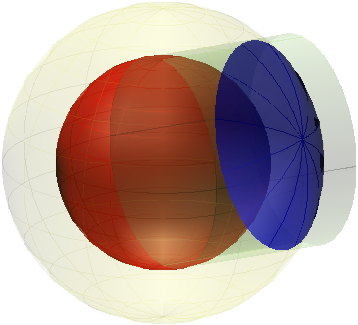
\includegraphics[width=.6\textwidth]{ombre.pdf}
    \caption{Proportion de zone observable pendant un an}
 \end{figure}
  
\end{frame}

\begin{frame}
\frametitle{Modélisation des saisons}

Les saisons sont déterminées par une variation de l'angle d'incidence entre le plan équatorial et les rayons solaires.\\


On modélise dans notre repère cette variation par $i_{soleil}(t)= i_{max}\cos(\omega_{s}t)$ où $i_{max}=23.75^o$ et $\displaystyle{\omega_s=\frac{2\pi}{T_s}}$.
\end{frame}

\begin{frame}
\frametitle{Modélisation des saisons}
 
\definecolor{uququq}{rgb}{0.25,0.25,0.25}
\definecolor{xdxdff}{rgb}{0.49,0.49,1}
\definecolor{qqqqff}{rgb}{0,0,1}
\begin{tikzpicture}[line cap=round,line join=round,>=triangle 45,x=1.0cm,y=1.0cm,scale=0.7]
\draw[->,color=black] (-5.43,0) -- (7.49,0);
\foreach \x in {-5,-4,-3,-2,-1,1,2,3,4,5,6,7}
\draw[shift={(\x,0)},color=black] (0pt,2pt) -- (0pt,-2pt) node[below] {\footnotesize $\x$};
\draw[->,color=black] (0,-3.62) -- (0,5.07);
\foreach \y in {-3,-2,-1,1,2,3,4,5}
\draw[shift={(0,\y)},color=black] (2pt,0pt) -- (-2pt,0pt) node[left] {\footnotesize $\y$};
\draw[color=black] (0pt,-10pt) node[right] {\footnotesize $0$};
\clip(-5.43,-3.62) rectangle (7.49,5.07);
\draw(0,0) circle (3cm);
\draw(0,0) circle (2cm);
\draw [domain=-5.43:7.49] plot(\x,{(-0--1.87*\x)/0.72});
\draw [domain=-5.43:7.49] plot(\x,{(-0--1.28*\x)/1.54});
\draw [domain=-5.43:7.49] plot(\x,{(-4--0.72*\x)/-1.87});
\draw [domain=-5.43:7.49] plot(\x,{(--4--0.72*\x)/-1.87});
\draw [domain=-5.43:7.49] plot(\x,{(-0--0.72*\x)/-1.87});
\draw [domain=-5.43:7.49] plot(\x,{(--4.47-1.87*\x)/-0.72});
\begin{scriptsize}
\fill [color=qqqqff] (0,0) circle (1.5pt);
\draw[color=qqqqff] (-0.13,0.25) node {$O$};
\fill [color=xdxdff] (1.54,1.28) circle (1.5pt);
\draw[color=xdxdff] (1.64,1.45) node {$T$};
\fill [color=xdxdff] (0.72,1.87) circle (1.5pt);
\draw[color=xdxdff] (0.85,2.04) node {$N'$};
\fill [color=uququq] (0,2) circle (1.5pt);
\draw[color=uququq] (0.2,2.18) node {$N_1$};
\fill [color=uququq] (2.31,1.92) circle (1.5pt);
\draw[color=uququq] (2.41,2.1) node {$D$};
\fill [color=uququq] (0,-2) circle (1.5pt);
\draw[color=uququq] (0.1,-1.83) node {$S$};
\fill [color=uququq] (-0.72,-1.87) circle (1.5pt);
\draw[color=uququq] (-0.62,-1.7) node {$S'$};
\fill [color=uququq] (2.81,1.06) circle (1.5pt);
\draw[color=uququq] (2.92,1.23) node {$X$};
\fill [color=uququq] (2.09,-0.81) circle (1.5pt);
\draw[color=uququq] (2.21,-0.63) node {$M$};
\end{scriptsize}
\end{tikzpicture}
\end{frame}

\begin{frame}
\frametitle{Conditions d'éclairement}
  
  \begin{figure}[h]
    \centering
    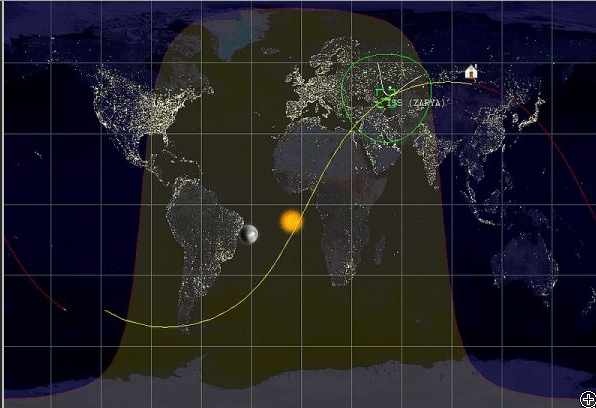
\includegraphics[width=.6\textwidth]{map2.png}
    \caption{Zone de jour}
 \end{figure}
\end{frame}

\begin{frame}
\frametitle{Portion de ciel observable}
 
\definecolor{qqwuqq}{rgb}{0,0.39,0}
\definecolor{uququq}{rgb}{0.25,0.25,0.25}
\definecolor{xdxdff}{rgb}{0.49,0.49,1}
\definecolor{qqqqff}{rgb}{0,0,1}
\begin{tikzpicture}[line cap=round,line join=round,>=triangle 45,x=1.0cm,y=1.0cm,scale=0.7]
\draw[->,color=black] (-5.76,0) -- (6.47,0);
\foreach \x in {-5,-4,-3,-2,-1,1,2,3,4,5,6}
\draw[shift={(\x,0)},color=black] (0pt,2pt) -- (0pt,-2pt) node[below] {\footnotesize $\x$};
\draw[->,color=black] (0,-4.44) -- (0,3.78);
\foreach \y in {-4,-3,-2,-1,1,2,3}
\draw[shift={(0,\y)},color=black] (2pt,0pt) -- (-2pt,0pt) node[left] {\footnotesize $\y$};
\draw[color=black] (0pt,-10pt) node[right] {\footnotesize $0$};
\clip(-5.76,-4.44) rectangle (6.47,3.78);
\draw [shift={(0,0)},color=qqwuqq,fill=qqwuqq,fill opacity=0.1] (0,0) -- (0:0.7) arc (0:22:0.7) -- cycle;
\draw(0,0) circle (3cm);
\draw(0,0) circle (2cm);
\draw [domain=-5.76:6.47] plot(\x,{(-0-0*\x)/2});
\draw (2.78,-4.44) -- (2.78,3.78);
\draw (0,0)-- (2.78,1.12);
\draw (0,0)-- (2.78,-1.12);
\begin{scriptsize}
\fill [color=qqqqff] (0,0) circle (1.5pt);
\draw[color=qqqqff] (-0.12,0.24) node {$O$};
\fill [color=xdxdff] (2,0) circle (1.5pt);
\draw[color=xdxdff] (2.1,0.16) node {$T$};
\fill [color=uququq] (0,2) circle (1.5pt);
\draw[color=uququq] (0.2,2.16) node {$N_1$};
\fill [color=uququq] (3,0) circle (1.5pt);
\draw[color=uququq] (3.1,0.16) node {$D$};
\fill [color=uququq] (0,-2) circle (1.5pt);
\draw[color=uququq] (0.09,-1.84) node {$S$};
\fill [color=xdxdff] (2.78,1.12) circle (1.5pt);
\draw[color=xdxdff] (2.88,1.28) node {$A$};
\fill [color=uququq] (2.78,-1.12) circle (1.5pt);
\draw[color=uququq] (2.87,-0.96) node {$B$};
\draw[color=qqwuqq] (0.56,0.11) node {$\beta$};
\end{scriptsize}
\end{tikzpicture} 
\end{frame}

\begin{frame}
\frametitle{Portion de ciel observable}
 
\definecolor{qqwuqq}{rgb}{0,0.39,0}
\definecolor{uququq}{rgb}{0.25,0.25,0.25}
\definecolor{xdxdff}{rgb}{0.49,0.49,1}
\definecolor{qqqqff}{rgb}{0,0,1}
\begin{tikzpicture}[line cap=round,line join=round,>=triangle 45,x=1.cm,y=1.cm,scale=0.6]
\draw[->,color=black] (-5.76,0) -- (6.47,0);
\foreach \x in {-5,-4,-3,-2,-1,1,2,3,4,5,6}
\draw[shift={(\x,0)},color=black] (0pt,2pt) -- (0pt,-2pt) node[below] {\footnotesize $\x$};
\draw[->,color=black] (0,-4.44) -- (0,3.78);
\foreach \y in {-4,-3,-2,-1,1,2,3}
\draw[shift={(0,\y)},color=black] (2pt,0pt) -- (-2pt,0pt) node[left] {\footnotesize $\y$};
\draw[color=black] (0pt,-10pt) node[right] {\footnotesize $0$};
\clip(-5.76,-4.44) rectangle (6.47,3.78);
\draw [shift={(0,0)},color=qqwuqq,fill=qqwuqq,fill opacity=0.1] (0,0) -- (63.02:0.64) arc (63.02:90:0.64) -- cycle;
\draw(0,0) circle (3cm);
\draw (0,0)-- (1.36,2.67);
\draw (1.36,-4.44) -- (1.36,3.78);
\draw (0,0)-- (1.36,-2.67);
\begin{scriptsize}
\fill [color=qqqqff] (0,0) circle (1.5pt);
\draw[color=qqqqff] (-0.12,0.24) node {$O$};
\fill [color=xdxdff] (1.36,2.67) circle (1.5pt);
\draw[color=xdxdff] (1.47,2.84) node {$A$};
\fill [color=uququq] (1.36,-2.67) circle (1.5pt);
\draw[color=uququq] (1.46,-2.51) node {$B$};
\fill [color=uququq] (0,3) circle (1.5pt);
\draw[color=uququq] (0.11,3.17) node {$C$};
\draw[color=qqwuqq] (0.26,0.39) node {$\delta$};
\end{scriptsize}
\end{tikzpicture} 
\end{frame}

\begin{frame}
\frametitle{Optimisation en fonction de la latitude}

\begin{itemize}
\item $\displaystyle{\beta(t)=\arccos\left(\frac{\sqrt{2rR+r^2}\cos(i_s(t))}{(R+r)\sin(\varphi)}\right)}$.
\item $\displaystyle{\delta(t)=\arcsin\left(\frac{|\tan(i_s(t))|}{\tan(\varphi)}\right)}$.
\item Proportion : $\displaystyle{p_{V}(t,\varphi)=\frac{(2\pi-2\beta(t))}{2\pi}\frac{(\frac{\pi}{2}-\delta(t))}{\pi}}$
\item On optimise la proportion moyenne $$p_{M}= \frac 1 {1 \text{ an}}\int_{\text{1 an}} p_{V}(t) \dd t$$
\end{itemize}



  
\end{frame}

\begin{frame}
\frametitle{Tracé de l'optimisé}


 \begin{figure}[h]
    \centering
    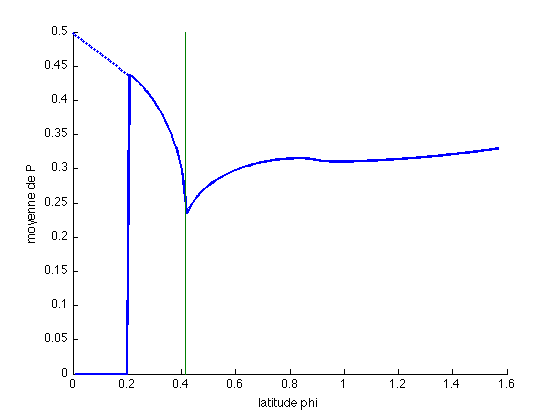
\includegraphics[width=.6\textwidth]{opt.png}
    \caption{Proportion de zone observable pendant un an}
 \end{figure}

  
\end{frame}

\begin{frame}
\frametitle{Variation d'observabiilité}


 \begin{figure}[h]
    \centering
    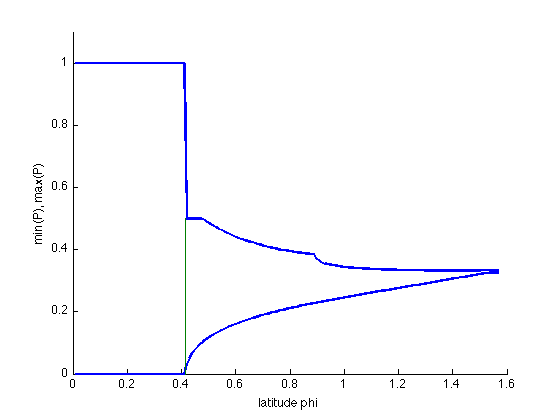
\includegraphics[width=.6\textwidth]{ecart.png}
    \caption{Variation d'éclairement suivant la latitude}
 \end{figure}

  
\end{frame}

% % On suppose que ça intervient juste par une proba indépendante chaque jour
% \frame{
%   \frametitle{Trucs à dire}
%   \begin{itemize}
%   \item Indépendance de la visibilité supposée
%   \item Héliosynchronisme : peut casser l'indépendance. En une
%     journée, dérive $T_{\text{terre}} \Delta\omega_{s}$, à comparer
%     avec $\alpha$ : passe $\alpha$ en un jour si $\Delta\omega_{s} \approx
%     10\%$, correspond à $\Delta a \approx 5\%$
%   \end{itemize}
% }
\section{Résultats}
\frame{
  \frametitle{Résultats}
  \begin{itemize}
  \item En un jour, si un débris est placé aléatoirement sur une
    orbite d'inclinaison $i_{D}$, on l'observe avec probabilité
    \begin{align*}
      p = 2 \times \frac {2\alpha} {2\pi} \times \frac
      {T_{\text{terre}}}{T_{\text{débris}} \sin {i_{D}}} \times p_{V}(\varphi,i_{D},t)\approx 1\%
    \end{align*}
  \item $n$ débris, $q$ téléscopes (suffisamment espacés), $T$ jours d'observation
  \item Problème avec les débris héliosynchrones : si on ne les voit
    au jour $J$, on ne les voit pas au jour $J+1$. Il faut une
    déviation sur la période de rotation de l'ordre de 5\% pour éviter
    ce problème.
  \end{itemize}
}
\frame{
  \frametitle{Résultats}
  \begin{itemize}
  % \item En un jour, si un débris est placé aléatoirement sur une
  %   orbite d'inclinaison $i_{D}$, on l'observe avec probabilité
  %   \begin{align*}
  %     p = 2 \times \frac {2\alpha} {2\pi} \times \frac
  %     {T_{\text{terre}}}{T_{\text{débris}} \sin {i_{D}}} \times p_{V}(\varphi,i_{D},t)\approx 1\%
  %   \end{align*}
  % \item $n$ débris, $q$ téléscopes (suffisamment espacés), $T$ jours d'observation
  \item On suppose une ``ergodicité'' : indépendance des différentes observations
  \item $N$ nombre de débris vus suit une loi binomiale $B(p,nqT)$
     \begin{align*}
      P(N \geq 1) = 1 - (1-p)^{nqT}
    \end{align*}

  \item Pour observer un débris avec un téléscope, il faut 2 mois pour
    avoir 50\% de chances, 8 mois pour 90\%, 15 mois pour 99\%
  \item Pour observer un débris avec dix téléscopes, il faut une semaine pour
    avoir 50\% de chances, trois semaines pour 90\%, six semaines pour 99\%
  % \item Tests numériques de cette loi
  \end{itemize}
}
\section{Ergodicité}
\frame{
  \frametitle{Ergodicité}
  \begin{itemize}
  \item Problème modèle (on ignore la visibilité) : on observe une
    fois par jour l'orbite du débris, il se déplace d'un angle
    $\theta$ sur son orbite, phase initiale aléatoire.
  \item $\theta = 2\pi\frac{T_{\text{terre}}}{T_{\text{débris}} +
      T_{\text{précession}} \cos {i_{d}}} \approx 2\pi
    \frac{T_{\text{terre}}}{T_{\text{débris}}} \approx 14.1 \text{ tours}$
  \item $\theta_{n} = \theta_{0} + n \theta \mod 2\pi$, on observe le
    débris si $\theta_{n} \in [0,\alpha]$
  \item $N(n)$ nombre d'observations en $n$ itérations
  \item Si
    $\frac{\theta}{2\pi}$ est irrationnel, on prouve
  \begin{align*}
    \lim_{n\to\infty} \frac{N(n)}{n} = \frac{\alpha}{2\pi}
  \end{align*}
\item ``Loi des grand nombres''. Vitesse de convergence de cette
  limite ? Théorème central limite ? 
  \end{itemize}
}
\frame{
  \frametitle{Ergodicité}
  \begin{itemize}
  \item Approximation aléatoire : $\theta = U(0,2\pi)$
  \item $N(n) = B(n,\frac \alpha {2\pi})$
  \item Temps caractéristique d'observation $n_{c}^{U}\approx
    \frac{2\pi}{\alpha}$
  \item $P(N(n) \geq 1) = 1 - (1 - \frac {\alpha}{2\pi})^{n}$
  \item Estimation pour le modèle déterministe ?
  \item On s'attend à ``$N(n) \geq 1$ pour $n$ de l'ordre de $\frac
    {2\pi}{\alpha}$ pour presque tout $\theta$'', mais on n'arrive pas
    à le prouver (bonne notion de ``de l'ordre de'' ? Cas où $\frac
    \theta {2\pi}$ est proche d'un rationnel ?)
  \item Tests numériques (très incomplets) : mitigé
  \end{itemize}
}
\section{Simulation}

\frame{
\frametitle{Mouvement de débris (Repère géocentrique)}
\begin{eqnarray}
   \Omega_O(t) = \Omega_O(t_0) + (t-t_0)\dot \Omega_O  \nonumber \\
   \Omega_D(t) = \Omega_D(t_0) + (t-t_0)\dot \Omega_D  \nonumber 
\end{eqnarray}
}

\frame{
\frametitle{Mouvement de débris}
\begin{center}
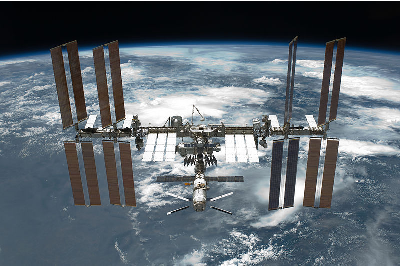
\includegraphics[width = 0.38\linewidth]{mks.pdf} \\
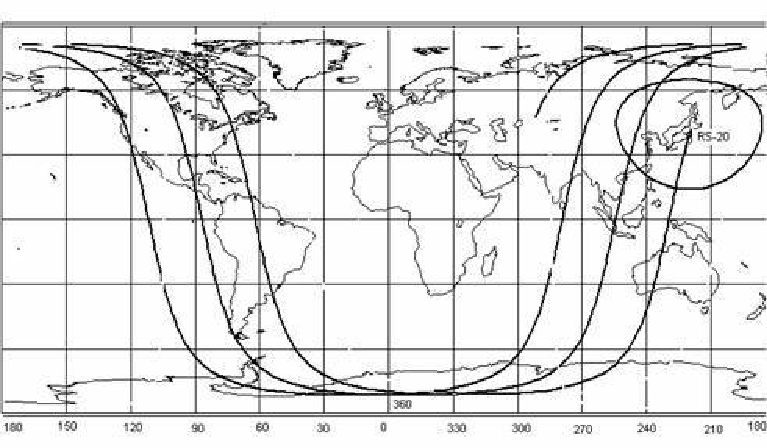
\includegraphics[width = 0.9\linewidth]{RS-20.pdf}
\end{center}



}


\frame{
\frametitle{Mouvement de débris et télescope}
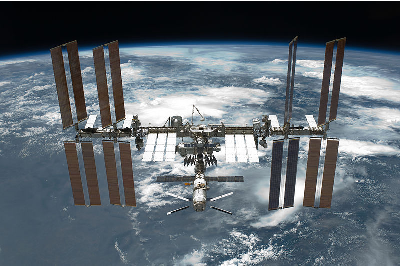
\includegraphics[width = 0.38\linewidth]{mks.pdf} \,
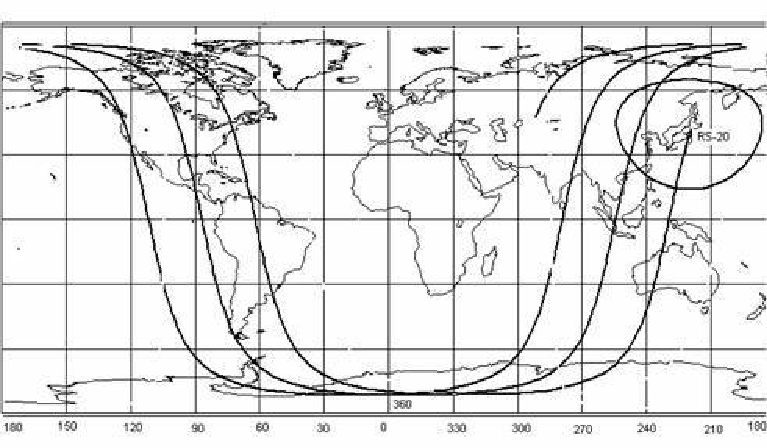
\includegraphics[width = 0.58\linewidth]{RS-20.pdf}


\begin{eqnarray}
   \Omega_O(t) = \Omega_O(t_0) + (t-t_0)\dot \Omega_O \nonumber \\
   \Omega_D(t) = \Omega_D(t_0) + (t-t_0)\dot \Omega_D  \nonumber \\
    \Omega_T(t) = \Omega_T(t_0) + (t-t_0)\dot \Omega_T  \nonumber 
\end{eqnarray}
}

\frame{
\frametitle{Mouvement de débris et télescope}
\begin{center}
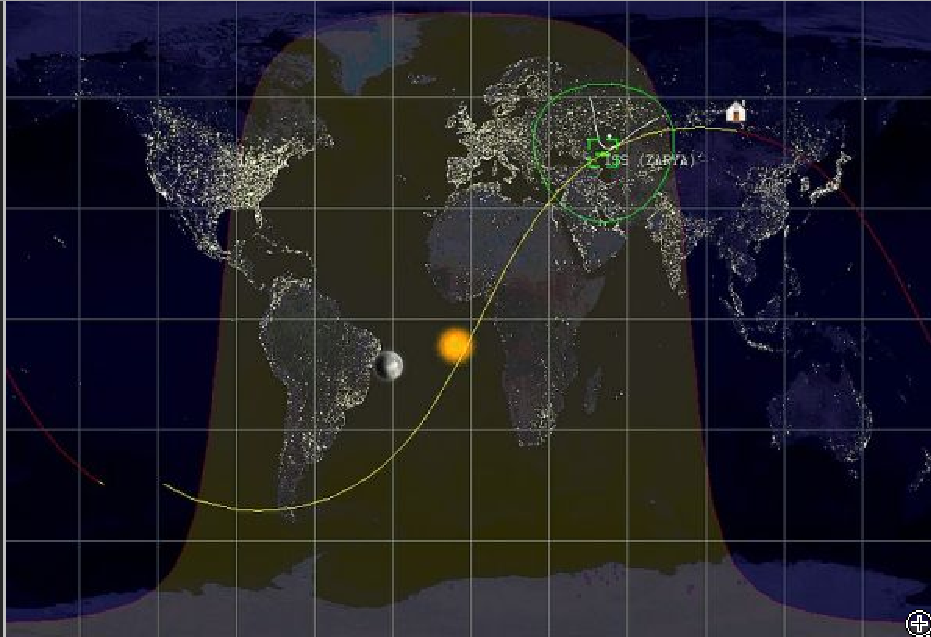
\includegraphics[width = 0.9\linewidth]{map2.pdf}  
\end{center}

}

\frame{
\frametitle{Mouvement de débris, télescope et Soleil}
\begin{center}
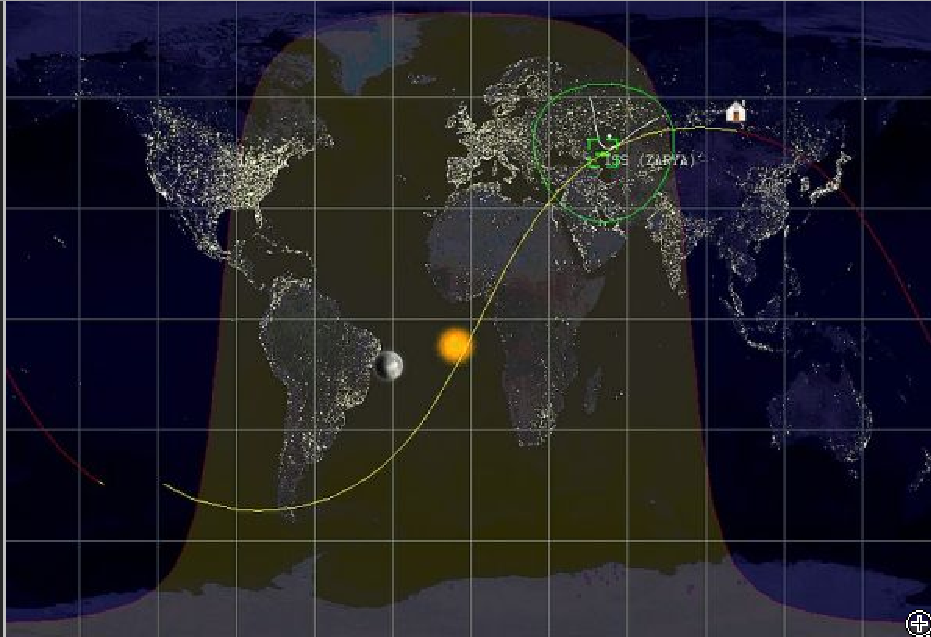
\includegraphics[width = 0.75\linewidth]{map2.pdf} 
\end{center}
\begin{eqnarray}
   \Omega_O(t) = \Omega_O(t_0) + (t-t_0)\dot \Omega_O  \nonumber \\
   \Omega_D(t) = \Omega_D(t_0) + (t-t_0)\dot \Omega_D  \nonumber \\
   \Omega_T(t) = \Omega_T(t_0) + (t-t_0)\dot \Omega_T  \nonumber \\
   \Omega_S(t) = \Omega_S(t_0) + (t-t_0)\dot \Omega_S  \nonumber 
\end{eqnarray}
}


\frame{
\frametitle{Mouvement de débris, télescopes et Soleil}
\begin{center}
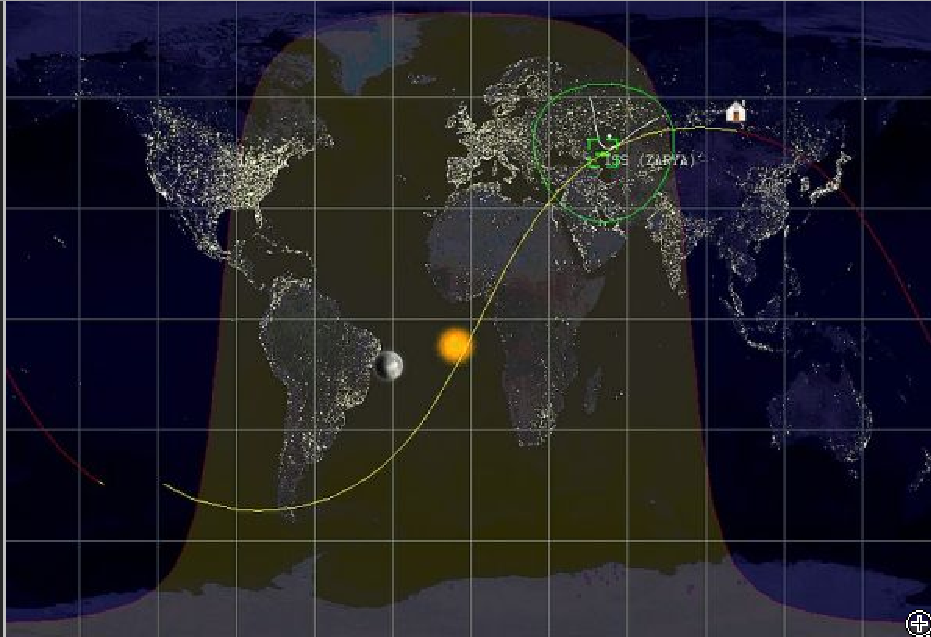
\includegraphics[width = 0.75\linewidth]{map2.pdf} 
\end{center}
\begin{eqnarray}
   \Omega_{O_i}(t) &=& \Omega_{O_i}(t_0) + (t-t_0)\dot \Omega_{O_i}  \nonumber \\
   \Omega_{D_i}(t) &=& \Omega_{D_i}(t_0) + (t-t_0)\dot \Omega_{D_i} , \, i = 1, \dots N \nonumber \\
   \Omega_{T_j}(t) &=& \Omega_{T_j}(t_0) + (t-t_0)\dot \Omega_{T_j} , \, j = 1, \dots M \nonumber \\
   \Omega_S(t) &=& \Omega_S(t_0) + \dot (t-t_0)\Omega_S  \nonumber 
\end{eqnarray}
}


\frame{
 \frametitle{Test d'érgodicité}
    $N = 100, 1000, 5000$
  
  Comparaison avec  $P \sim 1 - \left(1 - p \right)^{n}$.
  
  \pause
  
  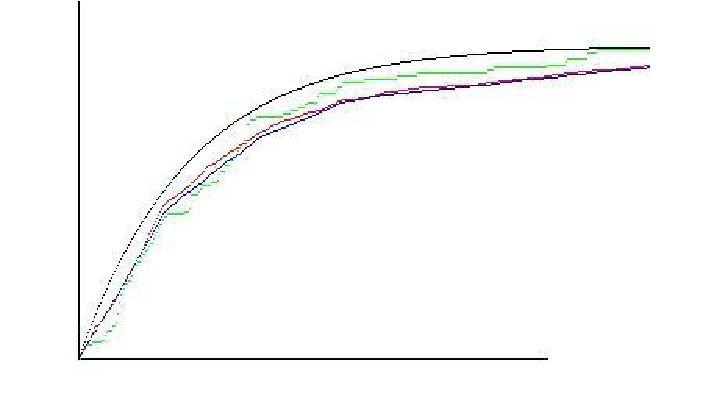
\includegraphics[width = 0.9\linewidth]{proba_obs.pdf}
  
  % {\small Calcul: cluster de l'ICJ Univ. Claude Bernard Lyon 1}
}

\frame{
\frametitle{Dépendence de nombre des télescopes}

\begin{center}
 
\begin{tabular}{|c|c|c|c|} \hline
 Débris & Téléscopes & Temps & \% vus \\ 
 \hline \hline
 100 & 10 & $\sim$ 2 mois &82 \\
 \hline
 100 & 2 & $\sim$ 10 mois &89 \\
 \hline
 \hline
 1000 & 10 & $\sim$ 2 mois &85.5 \\
 \hline
 1000 & 5 & $\sim$ 4 mois &86.7 \\
 \hline
 1000 & 2 & $\sim$ 10 mois &87.7 \\
 \hline  
 \hline
 10000 & 10 & $\sim$ 2 mois &84.0 \\
 \hline
 \hline
 $10^5$ & 14 & $\sim$ 8 mois & $\to 99$ \\
 \hline
\end{tabular} 
\end{center}
  % {\small Calcul: cluster de l'ICJ Univ. Claude Bernard Lyon 1}
\begin{itemize}
\item Cohérent avec $p \approx 1\%$, mais loi pas exactement binomiale
  : ergodicité approximative
\end{itemize}
}
\section{Conclusion}
\frame{
  \frametitle{Conclusion}
\begin{itemize}
\item Calculs rendus possibles par les échelles différentes mises en
  jeu (1 an / 1 jour, 1 jour / 2h)
\item Ordre de grandeur : 1\% par jour
\item Eclairage contribue un facteur moyen $1/2$, mais fortes
  variations saisonnières
\item Problèmes mathématiques (ergodicité)
\item Indépendance des observations : approximation correcte mais pas
  parfaite
\item Contexte physique : autres facteurs déterminant l'efficacité du
  téléscope (météo ...), possibilités et coûts d'installation, taille
  des débris ...
\end{itemize}
}
\end{document}
